% Chapter 5

\chapter{Comparative Analysis with FP Growth Algorithm} % Main chapter title

\label{Chapter1} % For referencing the chapter elsewhere, use \ref{Chapter1} 

\lhead{Chapter 5. \emph{Comparative Analysis with FP Growth Algorithm}} % This is for the header on each page - perhaps a shortened title

%----------------------------------------------------------------------------------------

\section{Applying FP Growth Algorithm: }

Since the objective of this step is comparison, not application of FP Growth, I will not go into detail about the application. 

I simply used the same encoded  \verb|DataFrame| from the last step (Apriori algorithm application) to apply FP Growth. FP Growth is also available in the \verb|mlxtend| Python library. The objective of FP Growth is the same as Apriori, hence it is a viable alternative. However, differences lie in the functionality, time complexity, memory usage and efficiency of both algorithms.

\newpage
\section{Comparison of Apriori and FP Growth Algorithms:}

\subsection{Functionality:}

\begin{table}[htbp]
    \centering
    \rowcolors{1}{pink!20}{white}
    \adjustbox{max width=\textwidth}{
    \begin{tabular}{|>{\columncolor{pink!50}}p{3cm}|p{6cm}|p{6cm}|}
        \hline
        \rowcolor{pink!50}
        \textbf{Feature/Aspect} & \textbf{Apriori} & \textbf{FP-Growth} \\
        \hline
        Candidate Generation & Uses a candidate generation and test approach. & Uses a compact FP-tree structure, avoids explicit candidate generation. \\
        Efficiency & Can be computationally expensive for large datasets. & Generally, more efficient, especially for large datasets. \\
        Support Counting & Requires multiple passes through the dataset. & Performs support counting in a single pass with FP-tree. \\
        Memory Usage & Can be memory-intensive due to storing candidates. & Generally, uses less memory with the compact FP-tree. \\
        Handling Sparse Data & Less efficient with sparse datasets. & Well-suited for sparse datasets due to FP-tree structure. \\
        Parallelization & Challenging to parallelize due to iterative nature. & Challenging to parallelize due to iterative nature. More amenable to parallelization, suitable for distributed computing. \\
        Algorithmic Complexity & Exponential worst-case complexity. & Better average-case performance.\\
        \hline
    \end{tabular}
    }
    \caption{There were no duplicates or outliers}
    \label{tab:pink_table_fit}
\end{table}

\subsection{Time Complexity:}
\begin{table}[htbp]
    \centering
    \rowcolors{1}{green!20}{white}
    \begin{tabular}{|>{\columncolor{green!50}}c|c|c|c|}
        \hline
        \rowcolor{green!50}
        \textbf{Algorithm} & \textbf{Total Time} & \textbf{Frequent Itemsets} & \textbf{Association Rule} \\
        \hline
        Apriori & 0.044761 & 0.043750 & 0.008000 \\
        FP Growth & 0.011839 & 0.008003 & 0.008027 \\
        \hline
    \end{tabular}
    % \caption{3 by 4 table with green color}
    \label{tab:3x4_green}
\end{table}


\begin{figure}[h]
    \centering
    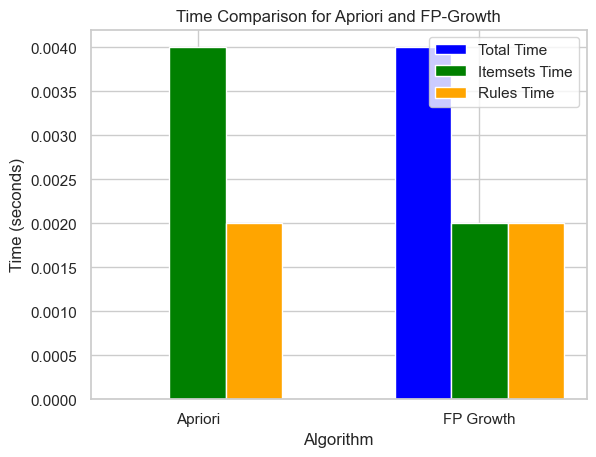
\includegraphics[width=0.7\textwidth]{Chapters/ch5/ch_5_bargraph.png}
    % \caption{Apriori graph}
    % \label{fig:example}
\end{figure}
\newpage
This graph shows how the total time for both processes (generating frequent itemsets and rule mining), just the time for frequent itemset generation, and just the time for association rule mining, differ from one another.


\subsection{Memory Usage:}

\begin{table}[htbp]
    \centering
    \rowcolors{1}{orange!20}{white}
    \renewcommand{\arraystretch}{1} % Adjust row height
    \begin{adjustbox}{max width=\textwidth}
    \begin{tabular}{|>{\columncolor{orange!50}}c|c|c|c|}
        \hline
        \rowcolor{orange!50}
        \textbf{Line\#} & \textbf{Memory Usage} & \textbf{Increment} & \textbf{Occurances} \\
        \hline
        41 & 142.1 MiB & 142.1 MiB & 1 \\
        42 &  &  & \\
        44 & 142.2 MiB & 0.1 MiB & 2 \\
        46 & 142.3 MiB & 0.0 MiB & 2 \\
        \hline
    \end{tabular}
    \end{adjustbox}
    \caption{Apriori}
    \label{tab:5x5_orange}
\end{table}

\begin{table}[htbp]
    \centering
    \rowcolors{1}{orange!20}{white}
    \renewcommand{\arraystretch}{1} % Adjust row height
    \begin{adjustbox}{max width=\textwidth}
    \begin{tabular}{|>{\columncolor{orange!50}}c|c|c|c|}
        \hline
        \rowcolor{orange!50}
        \textbf{Line\#} & \textbf{Memory Usage} & \textbf{Increment} & \textbf{Occurances} \\
        \hline
        53 & 142.3 MiB & 142.3 MiB & 1 \\
        54 &  &  & \\
        56 & 142.3 MiB & 0.0 MiB & 2 \\
        58 & 142.3 MiB & 0.0 MiB & 2 \\
        \hline
    \end{tabular}
    \end{adjustbox}
    \caption{Apriori}
    \label{tab:5x5_orange}
\end{table}


Both algorithms show minimal memory usage variations during their execution.
FP-Growth maintains a constant memory usage throughout its execution, indicating its ability to efficiently handle memory resources, especially for large datasets.
Apriori exhibits a slightly higher memory increment during the discovery of frequent itemsets, but the additional memory is modest and may not be a significant concern

% ----------------------------------------------------------------------------------------------------------------

\subsection{Summarized Differences:}

\begin{table}[htbp]
    \centering
    \rowcolors{2}{pink!20}{white}
    \begin{tabular}{|>{\bfseries\raggedright\arraybackslash}p{3cm}|>{\raggedright\arraybackslash}p{3cm}|>{\raggedright\arraybackslash}p{3cm}|>{\raggedright\arraybackslash}p{3cm}|}
        \hline
        \rowcolor{pink!80}
        {\textbf{Aspect}} & {\textbf{Apriori}} & {\textbf{FP-Growth}} & {\textbf{Empirical Evidence}} \\
        \hline
        Algorithmic Complexity & Generally, has higher algorithmic complexity, especially in the frequent itemset generation phase. & Lower algorithmic complexity due to a single-pass tree construction.& Apriori's complexity can lead to longer execution times, as seen in your data. \\
        Scalability & Tends to have scalability issues with large datasets and numerous itemsets. & More scalable, particularly for large datasets, as it requires fewer passes over the data. & FP-Growth may perform better as the dataset size increases, as suggested by your execution time results. \\
        Memory Requirements & Typically, higher memory requirements, especially when dealing with many transactions and items. & Lower memory requirements, especially for large datasets, as it constructs a compact FP-tree. & FP-Growth is expected to be more memory-efficient based on the provided data. \\
        Empirical Evidence & Apriori showed longer execution times, especially in the itemset generation phase. & FP-Growth demonstrated shorter execution times, indicating better performance. & The empirical evidence supports the idea that FP-Growth outperforms Apriori in terms of execution time. \\
        \hline
    \end{tabular}
    \caption{Table with 4 columns and 4 rows}
    \label{tab:4x4_sentences}
\end{table}
% \end{document}


